\documentclass{article}

\usepackage{graphicx}
\usepackage{tikz}
\usepackage{tikzsymbols}
\usetikzlibrary{calc,patterns,shapes.geometric}
\pagestyle{empty}
\usepackage[margin=0pt]{geometry}
\geometry{papersize={14in,12in}}

\def\centerarc[#1](#2)(#3:#4:#5){\draw[#1] ($(#2)+({#5*cos(#3)},{#5*sin(#3)})$) arc (#3:#4:#5);}

\begin{document}
	\begin{figure}
		\centering
		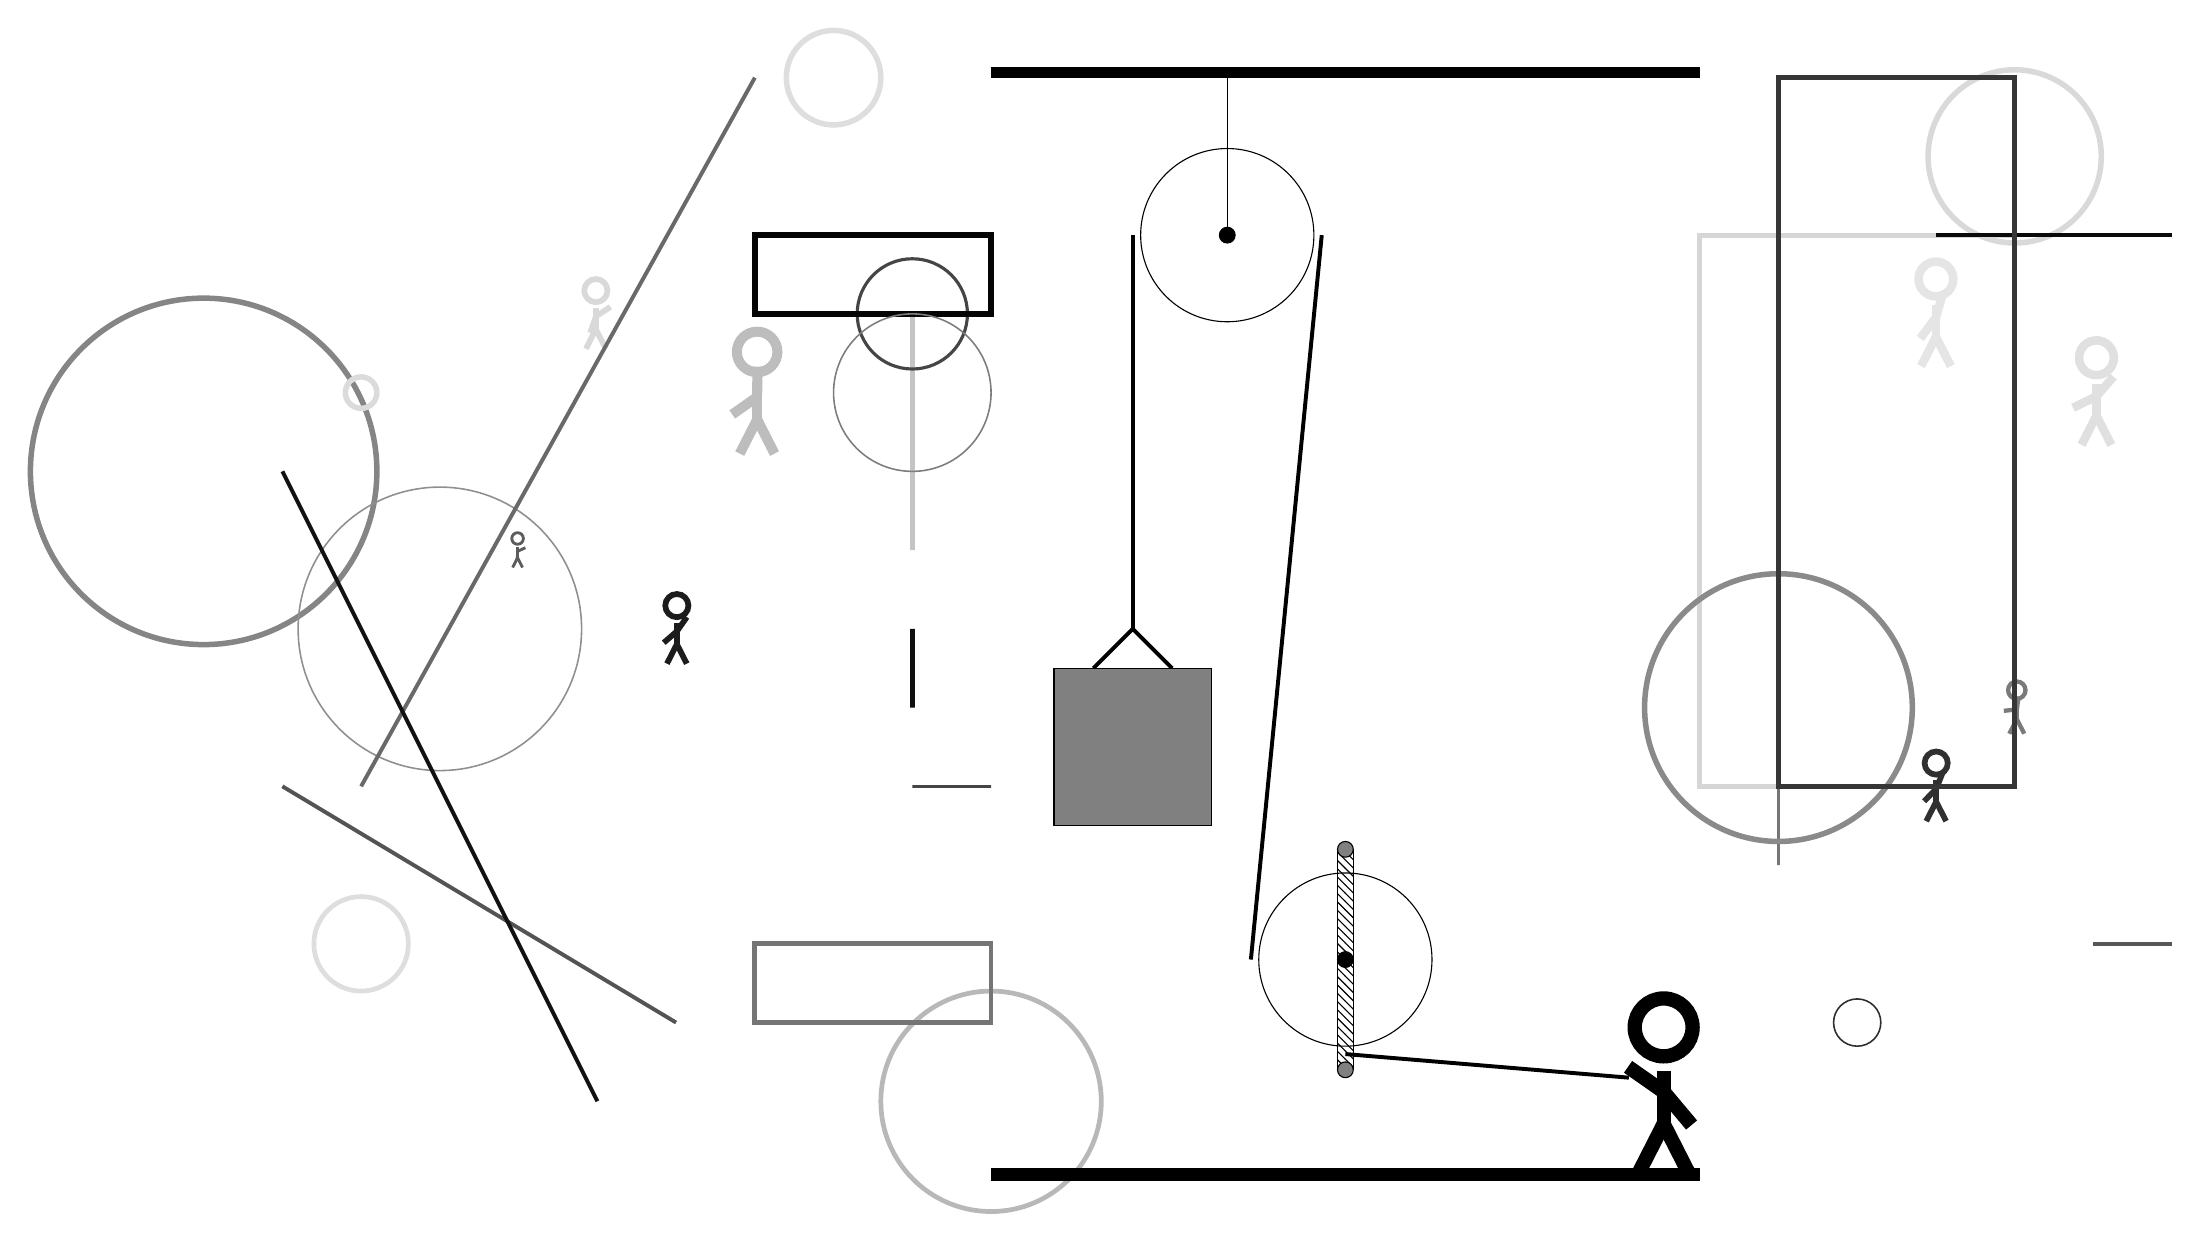
\begin{tikzpicture}
			%%%%% START %%%%%
			
			\draw[fill=black] (-2, 14) rectangle (7, 14.125);
			
			\draw (1, 12) circle (1.1);
			\draw[fill=black] (1, 12) circle (0.1);
			\draw (1, 14) -- (1, 12);
			
			\draw[fill=white](2.5, 2.8) circle (1.1);
			\draw[fill=black] (2.5, 2.8) circle (0.1);
			\draw[pattern=north west lines, pattern color=black] (2.4, 4.2) rectangle (2.6, 1.4);
			\draw[fill=black!50] (2.5, 4.2) circle (0.1);
			\draw[fill=black!50] (2.5, 1.4) circle (0.1);
			
			\node[line width=0.3mm, color=black!89] at (-6, 7) {\Strichmaxerl[4][41][55]};
			
			\draw[line width=0.3mm, color=black!54] (8, 4) rectangle (8, 13);
			\draw [line width=0.7mm, color=black!48](-12, 9) circle (2.2);
			\draw [line width=0.2mm, color=black!44](-9, 7) circle (1.8);
			\draw[line width=0.4mm, color=black!73] (-2, 5) rectangle (-3, 5);
			\draw[line width=0.6mm, color=black!16] (7, 5) rectangle (11, 12);
			\draw [line width=0.7mm, color=black!15](11, 13) circle (1.1);
			
			\draw[line width=0.6mm, color=black!23] (-3, 8) rectangle (-3, 11);
			\draw [line width=0.4mm, color=black!73](-3, 11) circle (0.7);
			\draw [line width=0.7mm, color=black!13](-4, 14) circle (0.6);
			
			\draw[line width=0.5mm, color=black!96](10, 12) -- (13, 12);
			
			\draw[line width=0.7mm, color=black!98] (-2, 11) rectangle (-5, 12);
			\draw [line width=0.7mm, color=black!46](8, 6) circle (1.7);
			\node[line width=0.7mm, color=black!15] at (-7, 11) {\Strichmaxerl[4][71][33]};
			\draw [line width=0.6mm, color=black!13](-10, 3) circle (0.6);
			\draw [line width=0.6mm, color=black!28](-2, 1) circle (1.4);
			\node[line width=0.2mm, color=black!12] at (12, 10) {\Strichmaxerl[6][26][49]};
			\draw[line width=0.5mm, color=black!59](-5, 14) -- (-10, 5);
			\draw [line width=0.2mm, color=black!51](-3, 10) circle (1.0);
			\draw[line width=0.6mm, color=black!54] (-2, 3) rectangle (-5, 2);
			\node[line width=0.2mm, color=black!81] at (10, 5) {\Strichmaxerl[4][46][68]};
			\node[line width=0.4mm, color=black!10] at (10, 11) {\Strichmaxerl[6][53][74]};
			
			\node[line width=0.7mm, color=black!52] at (11, 6) {\Strichmaxerl[3][6][82]};
			\draw[line width=0.7mm, color=black!79] (8, 14) rectangle (11, 5);
			\node[line width=0.2mm, color=black!26] at (-5, 10) {\Strichmaxerl[7][35][89]};
			
			\draw[line width=0.5mm, color=black!67](-6, 2) -- (-11, 5);
			\draw[line width=0.5mm, color=black!66](12, 3) -- (13, 3);
			\node[line width=0.5mm, color=black!64] at (-8, 8) {\Strichmaxerl[2][88][25]};
			\draw[line width=0.7mm, color=black!94] (-3, 6) rectangle (-3, 7);
			\draw [line width=0.2mm, color=black!82](9, 2) circle (0.3);
			\draw [line width=0.7mm, color=black!14](-10, 10) circle (0.2);
			\draw[line width=0.5mm, color=black!93](-7, 1) -- (-11, 9);
			
			\draw[line width=0.5mm] (-0.7, 6.5) -- (-0.2, 7.0) -- (0.3, 6.5);
			\draw[fill=black!50] (-1.2, 6.5) rectangle (0.8, 4.5);
			
			\draw[line width=0.5mm] (-0.2, 12) -- (-0.2, 7.0);
			\centerarc[line width=0.5mm](1, 12)(0:180:1.2000000000000002);
			\draw[line width=0.5mm](2.2, 12) -- (1.3, 2.8);
			\centerarc[line width=0.5mm](2.5, 2.8)(180:270:1.2000000000000002);
			\draw[line width=0.5mm](2.5, 1.6) -- (6.1, 1.3);
			
			\node at (6.5, 1.2) {\Strichmaxerl[10][-35][-50]};
			
			\draw[fill=black] (-2, 0) rectangle (7, 0.15);
			
			%%%%% END %%%%%
		\end{tikzpicture}
	\end{figure}	
\end{document}